\begin{appendices}
\chapter{Project Planning}
\section{Project Timeline}
\begin{figure}[h]
\centering
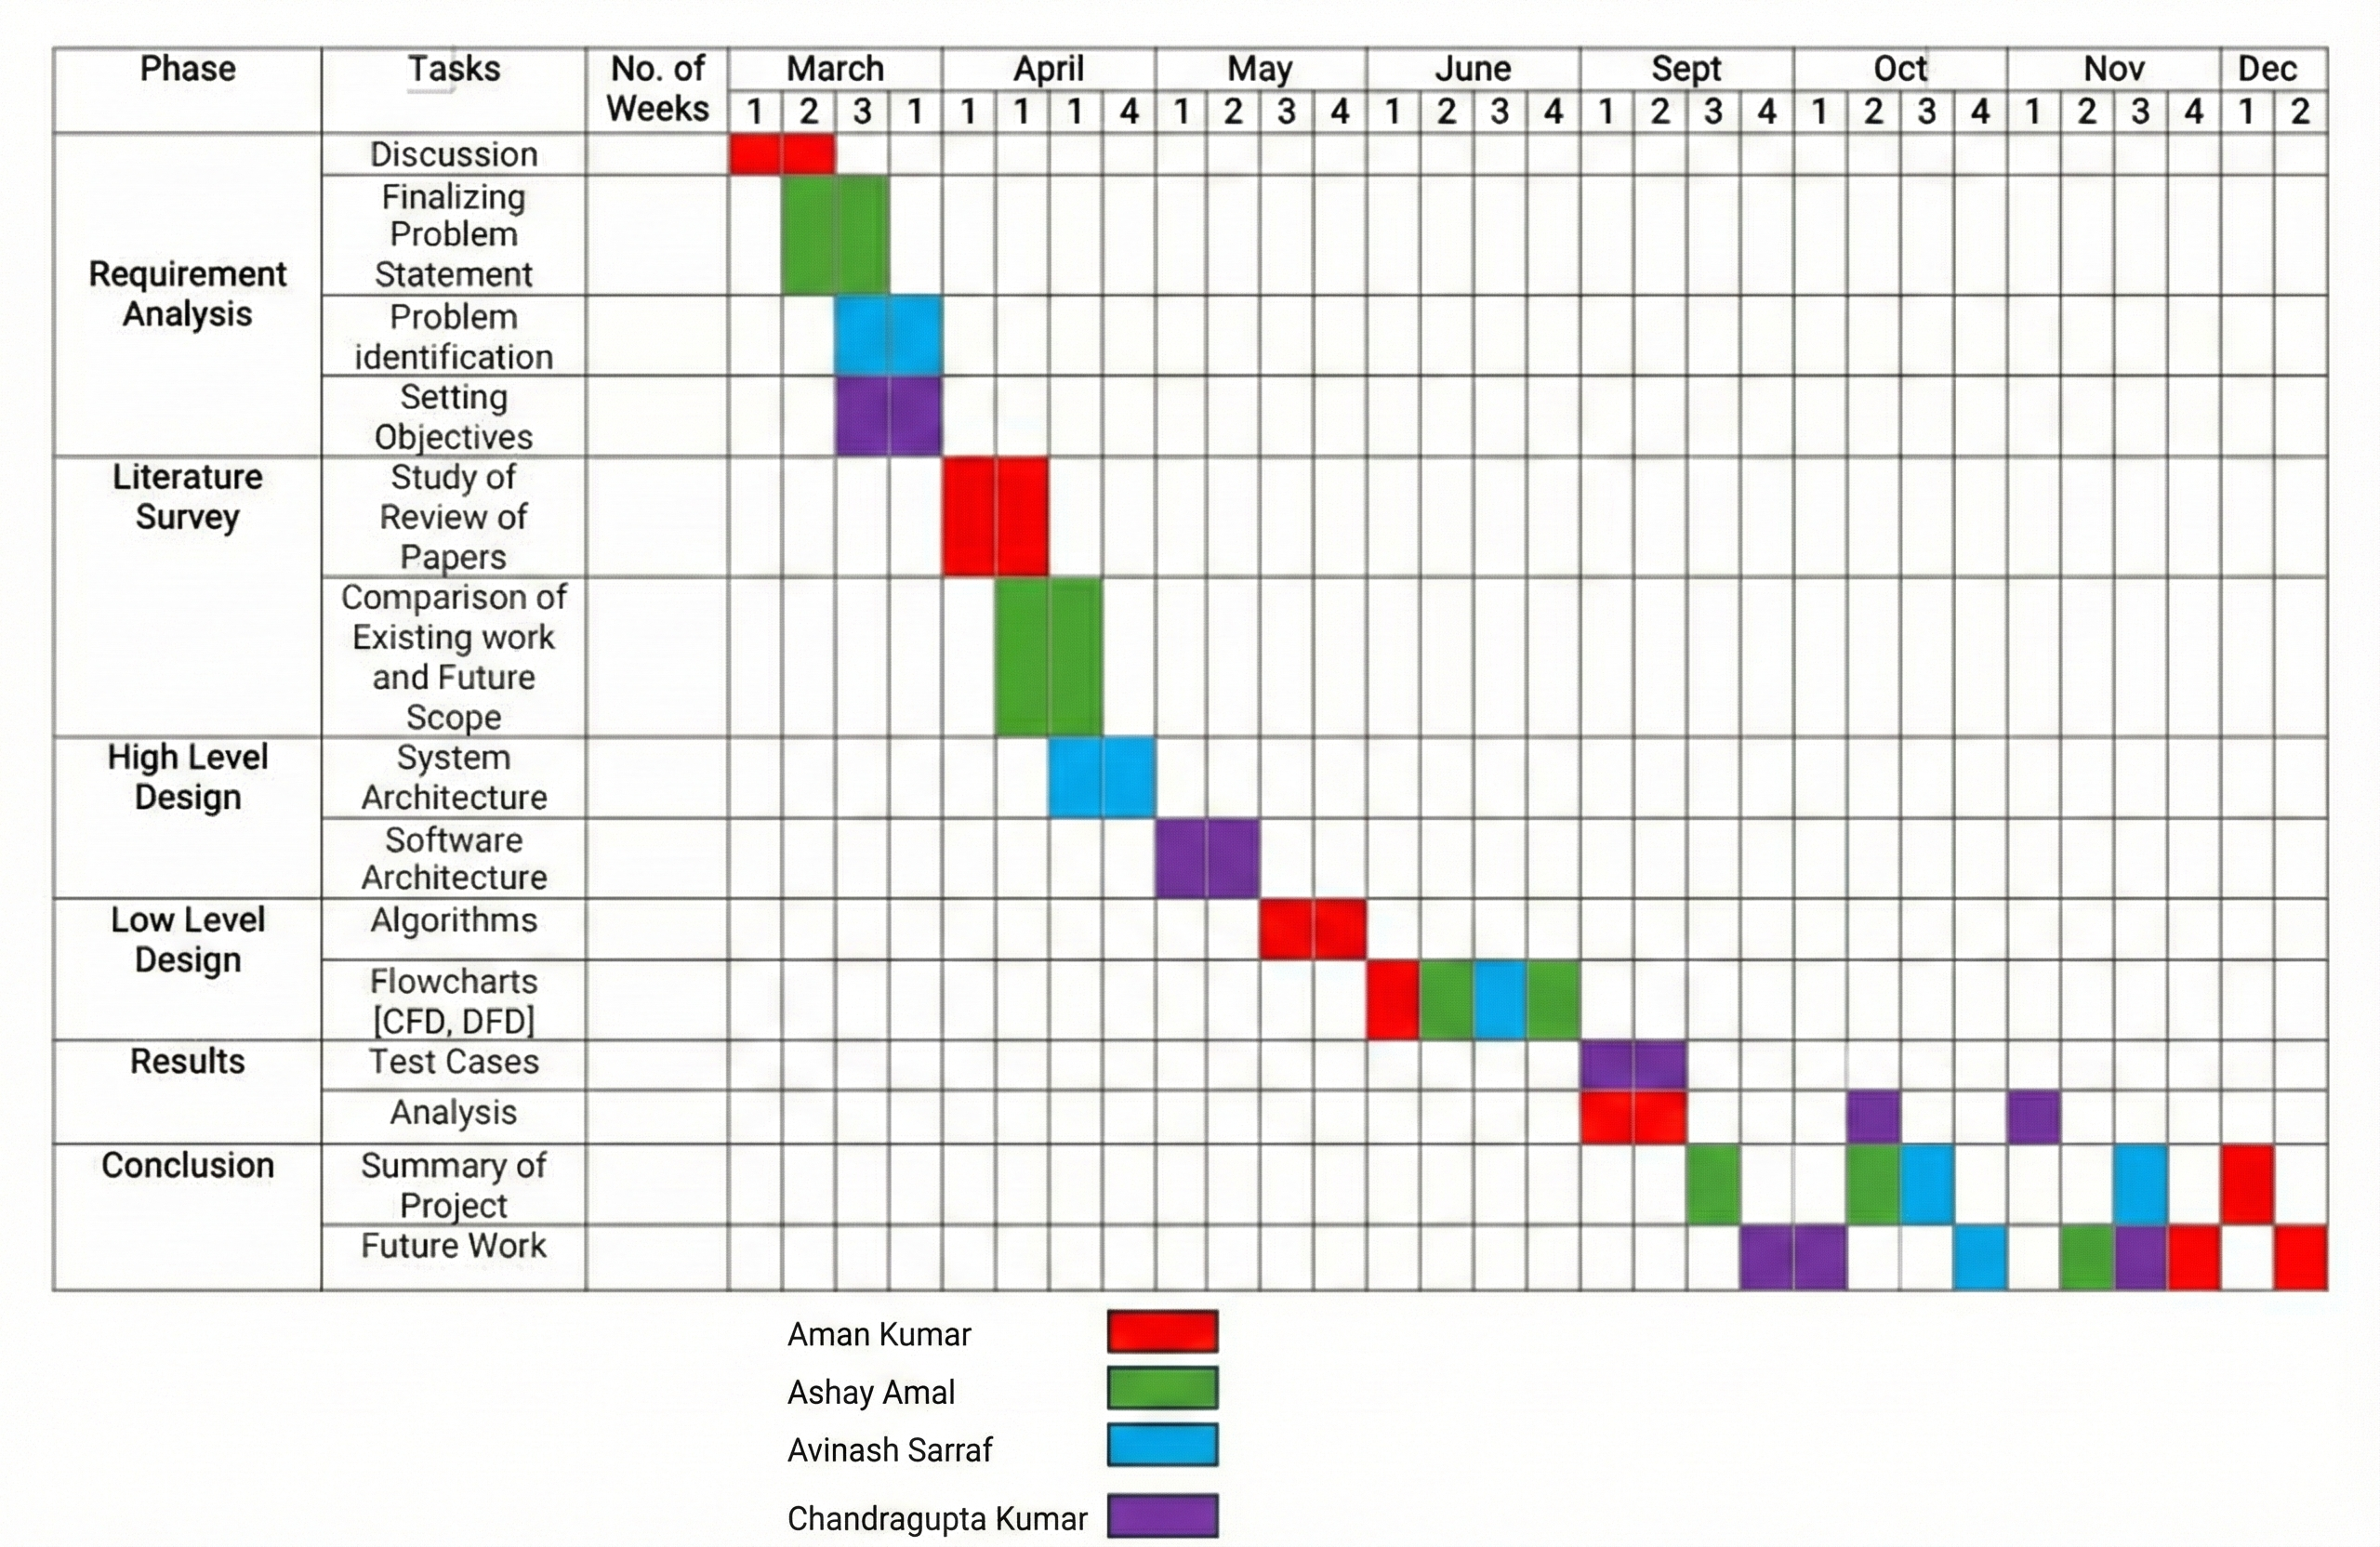
\includegraphics[width=\textwidth,height=1\textwidth]{timeline.png}
\caption{The Project Timeline.}
\label{fig:timeline}
\end{figure} 

\begin{table}[H]
\centering
\begin{tabular}{|l|l|l|}
\hline
\textbf{Phase} & \textbf{Activity} & \textbf{Duration} \\ \hline
Phase 1 & Literature Review \& Research & 2 weeks \\ \hline
Phase 2 & Dataset Collection \& Preparation & 3 weeks \\ \hline
Phase 3 & Model Architecture Implementation & 5 weeks \\ \hline
Phase 4 & Model Training \& Optimization & 4 weeks \\ \hline
Phase 5 & Testing, Evaluation \& Documentation & 2 weeks \\ \hline
\multicolumn{2}{|l|}{\textbf{Total Duration}} & \textbf{16 weeks} \\ \hline
\end{tabular}
\caption{Project Milestone Schedule}
\end{table}

\section{Budget Estimation}

\begin{table}[H]
\centering
\begin{tabular}{|l|l|r|}
\hline
\textbf{Category} & \textbf{Item} & \textbf{Cost (INR)} \\ \hline
\multirow{3}{*}{Hardware} & GPU Cloud Computing (Google Colab Pro) & 2,500 \\ \cline{2-3}
 & Storage (Cloud) & 200/month \\ \cline{2-3}
 & Miscellaneous Hardware & 2,000 \\ \hline
\multirow{2}{*}{Software} & Dataset (Kaggle - Free) & 0 \\ \cline{2-3}
 & Development Tools (Open Source) & 0 \\ \hline
\multirow{2}{*}{Other} & Documentation \& Printing & 1,500 \\ \cline{2-3}
 & Contingency & 1,500 \\ \hline
\multicolumn{2}{|l|}{\textbf{Total Estimated Cost (4 months)}} & \textbf{9,000} \\ \hline
\end{tabular}
\caption{Project Budget Estimation}
\end{table}

\chapter{Sustainable Development Goals (SDGs) Addressed}

\begin{longtable}{|p{8cm}|c|}
\hline
\textbf{SDG} & \textbf{Level} \\ \hline
No Poverty & 1 \\ \hline
Zero Hunger & 1 \\ \hline
Good Health and Well-being & 1 \\ \hline
Quality Education & 3 \\ \hline
Gender Equality & 2 \\ \hline
Clean Water and Sanitation & 1 \\ \hline
Affordable and Clean Energy & 1 \\ \hline
Decent Work and Economic Growth & 2 \\ \hline
Industry, Innovation and Infrastructure & 3 \\ \hline
Reduced Inequalities & 2 \\ \hline
Sustainable Cities and Communities & 2 \\ \hline
Responsible Consumption and Production & 2 \\ \hline
Climate Action & 1 \\ \hline
Life Below Water & 1 \\ \hline
Life on Land & 1 \\ \hline
Peace, Justice and Strong Institutions & 1 \\ \hline
Partnerships for the Goals & 2 \\ \hline
\end{longtable}
\textbf{Levels:} Poor = 1, Good = 2, Excellent = 3


\chapter{Self-Assessment of the Project}

\begin{longtable}{|p{1cm}|p{7cm}|p{5cm}|p{1.5cm}|}
\hline
\textbf{No.} & \textbf{PO and PSO} & \textbf{Contribution from the project} & \textbf{Level} \\ \hline

1 & \textbf{Engineering Knowledge:} Knowledge of mathematics, engineering fundamentals, and engineering specialization to form solutions for complex engineering problems. & Applied deep learning mathematics, loss functions, optimization algorithms & 3 \\ \hline

2 & \textbf{Problem Analysis:} Identify, formulate, review research literature, and analyze complex engineering problems to reach substantiated conclusions. & Conducted literature survey, identified research gaps, formulated solution approach & 3 \\ \hline

3 & \textbf{Design/development of solutions:} Design creative solutions for complex engineering problems. & Designed CycleGAN architecture with custom improvements for style transfer & 3 \\ \hline

4 & \textbf{Conduct investigations of complex problems:} Conduct investigations using research-based knowledge. & Experimented with different architectures, loss functions, and hyperparameters & 3 \\ \hline

5 & \textbf{Modern tool usage:} Create, select, and apply appropriate techniques, resources, and modern engineering \& IT tools. & Used PyTorch, CUDA, OpenCV, and modern deep learning tools & 3 \\ \hline

6 & \textbf{The Engineer and the world:} Analyze and evaluate societal and environmental impacts. & Considered applications in education, entertainment, and creative industries & 2 \\ \hline

7 & \textbf{Ethics:} Apply ethical principles; commit to professional ethics. & Used publicly available datasets, cited all references appropriately & 2 \\ \hline

8 & \textbf{Individual and Team Work:} Function effectively as an individual and as a member in diverse teams. & Collaborated on different aspects: dataset creation, model training, documentation & 3 \\ \hline

9 & \textbf{Communication:} Communicate effectively within the engineering community. & Prepared comprehensive documentation, created visualizations and diagrams & 3 \\ \hline

10 & \textbf{Project Management and Finance:} Apply engineering management principles. & Planned project phases, managed timeline, estimated budget & 2 \\ \hline

11 & \textbf{Life-long Learning:} Recognize the need for independent and life-long learning. & Learned new deep learning techniques, stayed updated with recent research & 3 \\ \hline

12 & \textbf{PSO1 – Computer-based systems development:} Design computer-based systems. & Developed complete neural network system for image transformation & 3 \\ \hline

13 & \textbf{PSO2 – Software development:} Specify, design, and develop applications. & Implemented training and inference pipelines using best practices & 3 \\ \hline

14 & \textbf{PSO3 – Computer communications and Internet applications:} Design network applications. & System can be deployed as web service with REST API & 2 \\ \hline

\end{longtable}
\textbf{Levels:} Poor = 1, Good = 2, Excellent = 3

\chapter{Dataset Details}

Detailed dataset information is provided in Chapter 3 (System Overview). The summary statistics are shown below:

\begin{table}[H]
\centering
\begin{tabular}{|l|c|c|c|l|}
\hline
\textbf{Style} & \textbf{Domain X} & \textbf{Domain Y} & \textbf{Total} & \textbf{Source} \\ \hline
One Piece & 3,000+ & 2,500+ & 5,500+ & Episodes \\ \hline
Disney & 3,000+ & 2,000+ & 5,000+ & Movies \\ \hline
Studio Ghibli & 3,000+ & 2,000+ & 5,000+ & Films \\ \hline
Van Gogh & 2,500+ & 400+ & 2,900+ & Kaggle Datasets \\ \hline
Human Faces & 3,000+ & 2,000+ & 5,000+ & Kaggle \\ \hline
Landscape Images & 3,000+ & 2,000+ & 5,000+ & Kaggle \\ \hline
\textbf{Total} & \textbf{11,500+} & \textbf{6,900+} & \textbf{18,400+} & -- \\ \hline
\end{tabular}
\caption{Complete Dataset Statistics}
\end{table}

All images are preprocessed to 256$\times$256 pixels in RGB format with normalization to [-1, 1] range.

\chapter{Configuration and Usage}

\section{Repository Structure}

The source code is organized in a modular structure to facilitate understanding, modification, and extension:

\begin{table}[H]
\centering
\begin{tabular}{|l|p{9cm}|}
\hline
\textbf{Directory/File} & \textbf{Description} \\ \hline
\texttt{models/} & Neural network architecture definitions \\ \hline
\quad \texttt{generator.py} & ResNet-based generator with 9 residual blocks \\ \hline
\quad \texttt{discriminator.py} & PatchGAN discriminator implementation \\ \hline
\quad \texttt{cyclegan.py} & Complete CycleGAN model with training logic \\ \hline
\texttt{utils/} & Utility functions and helper modules \\ \hline
\quad \texttt{dataset.py} & Custom PyTorch Dataset class for unpaired data \\ \hline
\quad \texttt{transforms.py} & Image preprocessing and augmentation \\ \hline
\quad \texttt{losses.py} & Loss function implementations (perceptual, cycle) \\ \hline
\quad \texttt{buffer.py} & Image history buffer for discriminator training \\ \hline
\texttt{train.py} & Training script with argument parsing \\ \hline
\texttt{inference.py} & Inference script for style transfer \\ \hline
\texttt{checkpoints/} & Saved model weights ($\sim$150 MB per style) \\ \hline
\texttt{data/} & Training datasets organized by style \\ \hline
\texttt{requirements.txt} & Python package dependencies \\ \hline
\end{tabular}
\caption{Project Directory Structure}
\end{table}
\newpage
\section{Installation Guide}

\subsection{Installation Steps}

\begin{enumerate}
    \item \textbf{Clone Repository:}
\begin{lstlisting}[language=bash]
git clone https://github.com/Ashay-Amal/cyclegan-style-transfer.git
cd cyclegan-style-transfer
\end{lstlisting}

    \item \textbf{Create Virtual Environment:}
\begin{lstlisting}[language=bash]
python -m venv venv
source venv/bin/activate  # Linux/Mac
# or: venv\Scripts\activate  # Windows
\end{lstlisting}

    \item \textbf{Install Dependencies:}
\begin{lstlisting}[language=bash]
pip install -r requirements.txt
\end{lstlisting}

    \item \textbf{Verify CUDA Installation:}
\begin{lstlisting}[language=python]
import torch
print(torch.cuda.is_available())  # Should print True
print(torch.cuda.get_device_name(0))
\end{lstlisting}
\end{enumerate}
\end{appendices}

